%%%%%%%%%%%%%%%%%%%%%%%%%%%%%%%%%%%%%%%%%
% Beamer Presentation
% LaTeX Template
% Version 1.0 (10/11/12)
%
% This template has been downloaded from:
% http://www.LaTeXTemplates.com
%
% License:
% CC BY-NC-SA 3.0 (http://creativecommons.org/licenses/by-nc-sa/3.0/)
%
%%%%%%%%%%%%%%%%%%%%%%%%%%%%%%%%%%%%%%%%%

%----------------------------------------------------------------------------------------
%   PACKAGES AND THEMES
%----------------------------------------------------------------------------------------

\documentclass{beamer}

\mode<presentation> {

% The Beamer class comes with a number of default slide themes
% which change the colors and layouts of slides. Below this is a list
% of all the themes, uncomment each in turn to see what they look like.

%\usetheme{default}
%\usetheme{AnnArbor}
%\usetheme{Antibes}
%\usetheme{Bergen}
%\usetheme{Berkeley}
%\usetheme{Berlin}
%\usetheme{Boadilla}
%\usetheme{CambridgeUS}
%\usetheme{Copenhagen}
%\usetheme{Darmstadt}
%\usetheme{Dresden}
%\usetheme{Frankfurt}
%\usetheme{Goettingen}
%\usetheme{Hannover}
%\usetheme{Ilmenau}
%\usetheme{JuanLesPins}
%\usetheme{Luebeck}
\usetheme{Madrid}
%\usetheme{Malmoe}
%\usetheme{Marburg}
%\usetheme{Montpellier}
%\usetheme{PaloAlto}
%\usetheme{Pittsburgh}
%\usetheme{Rochester}
%\usetheme{Singapore}
%\usetheme{Szeged}
%\usetheme{Warsaw}

% As well as themes, the Beamer class has a number of color themes
% for any slide theme. Uncomment each of these in turn to see how it
% changes the colors of your current slide theme.

%\usecolortheme{albatross}
%\usecolortheme{beaver}
%\usecolortheme{beetle}
%\usecolortheme{crane}
%\usecolortheme{dolphin}
%\usecolortheme{dove}
%\usecolortheme{fly}
%\usecolortheme{lily}
%\usecolortheme{orchid}
%\usecolortheme{rose}
%\usecolortheme{seagull}
%\usecolortheme{seahorse}
%\usecolortheme{whale}
%\usecolortheme{wolverine}

%\setbeamertemplate{footline} % To remove the footer line in all slides uncomment this line
\setbeamertemplate{footline}[page number] % To replace the footer line in all slides with a simple slide count uncomment this line

\setbeamertemplate{navigation symbols}{} % To remove the navigation symbols from the bottom of all slides uncomment this line
}

\usepackage{graphicx} % Allows including images
\usepackage{booktabs} % Allows the use of \toprule, \midrule and \bottomrule in tables
\usepackage{lmodern} % gets rid of font warnings
\usepackage{listings}
\usepackage[makeroom]{cancel}
\usepackage{algpseudocode}

%----------------------------------------------------------------------------------------
%   TITLE PAGE
%----------------------------------------------------------------------------------------

\title[Short title]{Generals Exam: Enhancing AlphaZero to Accomodate a Larger Policy Space and Applications} % The short title appears at the bottom of every slide, the full title is only on the title page

\author{Zachary Hervieux-Moore} % Your name
\date{18/05/18} % Date, can be changed to a custom date

\begin{document}

\begin{frame}
\titlepage % Print the title page as the first slide
\end{frame}

\begin{frame}
\frametitle{Overview} % Table of contents slide, comment this block out to remove it
\tableofcontents % Throughout your presentation, if you choose to use \section{} and \subsection{} commands, these will automatically be printed on this slide as an overview of your presentation
\end{frame}

%----------------------------------------------------------------------------------------
%   PRESENTATION SLIDES
%----------------------------------------------------------------------------------------

%------------------------------------------------
\section{Review \& Preliminaries} % Sections can be created in order to organize your presentation into discrete blocks, all sections and subsections are automatically printed in the table of contents as an overview of the talk
%------------------------------------------------

\subsection{Markov Decision Processes and Dynamic Programming} % A subsection can be created just before a set of slides with a common theme to further break down your presentation into chunks

%------------------------------------------------

\begin{frame}
  \frametitle{Markov Decision Processes}

  MDPs are 5-tuples consisting of $(S, A, P_{\cdot}(\cdot), R_{\cdot}(\cdot), \gamma)$
  \begin{itemize}
    \item $\mathcal{S}$ is the set of all states, $S_t \in S$ is a state at time $t$
    \item $\mathcal{A}$ is the set of all states, $a_t \in A$ is an action performed at time $t$
    \item $P_a(S_{t+1} | S_t)$ is the transition probability from state $S_t$ to the next state under action $a_t$
    \item $R_a(S_{t+1}, S_t)$ is the reward received after performing action $a_t$ in state $S_t$ and ending up in $S_{t+1}$
    \item $\gamma \in [0,1]$ is the discount factor on future rewards (how greedy you are)
  \end{itemize}
\end{frame}

%------------------------------------------------

%------------------------------------------------

\begin{frame}
  \frametitle{Dynamic Programming}

  \begin{itemize}
    \item Dynamic programming is the process of solving a complex problems by solving many simpler problems
    \item Backwards induction can be used to solve MDP finite horizon problem (finding best policy $\pi$ that maximizes reward)
      \begin{gather*}
        V_\pi(s) = \mathbb{E}[\sum_{t=0}^k R_\pi(s) | s, \pi]
      \end{gather*}
    \item Rich history of solving MDP infite horizon problems using Bellman equation and backwards induction on stochastic MDPs to get value iteration
      \begin{gather*}
        V_{i+1}(s) = \max_a \left\{ \sum_{s'} P_a(s' | s)(R_a(s',s)+\gamma V_i(s'))  \right\}
      \end{gather*}
  \end{itemize}
\end{frame}

%------------------------------------------------

\subsection{Multi-armed Bandit Theory}

\begin{frame}
  \frametitle{Multi-armed Bandit Problems}

  \begin{center}
    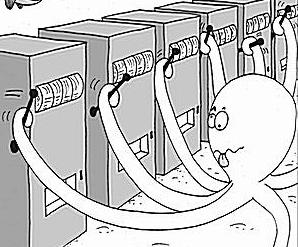
\includegraphics[width=0.3\linewidth]{./images/bandit.png}
  \end{center}

  \begin{itemize}
    \item $K$ machines that give out rewards according to some distribution in $[0,1]$
    \item $X_{i,n}$ is a random variable of the reward for pulling machine $i$ for the $n^{th}$ time
    \item Let $T_j(n)$ be the number of times machine $j$ is pulled after $n$ turns
    \item Regret:
      \begin{gather*}
        \mu^* n - \sum_i{K} \mu_j T_j(n)
      \end{gather*}
  \end{itemize}
\end{frame}

%------------------------------------------------

\begin{frame}
  \frametitle{Upper Confidence Bound}

  \begin{itemize}
    \item Algorithm that balances exploration vs. exploitation to achieve optimal asymptotic lower bound for regret
    \item Regret after $n$ rounds:
      \begin{gather*}
        O \left( \sqrt{K n \log(n)} \right)
      \end{gather*}
    \item Algorithm:
      \begin{gather*}
        \arg\max_j \bar{X_j} + \sqrt{\frac{2 \ln n}{n_j}}
      \end{gather*}
    \item Variant: if $P_1, \mathellipsis, P_K$ are probabilities of arms being optimal then regret becomes
      \begin{gather*}
        O \left( \sqrt{n \log(n)} (\sum_i \sqrt(P_i))^2 \right)
      \end{gather*}
  \end{itemize}
\end{frame}

%------------------------------------------------

%------------------------------------------------

\begin{frame}
  \frametitle{EXP3}

  \begin{itemize}
    \item Algorithm that also achieves the optimal regret lower bound but for the much more general case of adversarial multi-armed bandits
    \item Algorithm:
      \begin{algorithmic}
        \State $\gamma \in [0,1]$, $w_i(0) = 1$ for $i \in \{1, \mathellipsis, K\}$, $n=0$
        \While{$n < $ max\_iterations}
          \State 1) $p_i(n) \gets = (1-\gamma) \frac{w_i(n)}{\sum_{j=1}^K w_j(n)} + \frac{\gamma}{K}$
          \State 2) $a_n \sim$ distribution of $p_i(n)$'s
          \State 3) get reward $X_{a_n}(n)$
          \State 4) $\bar{X}_{a_n}(n) = X_{a_n}(n)/p_i(n)$
          \State 5) $w_i(n+1) = w_i(n) e^{\gamma \bar{X}_{a_n}(n)/K}$
          \State 6) $w_j(n+1) = w_j(n)$ for all other $j \neq i$
        \EndWhile
      \end{algorithmic}
  \end{itemize}
\end{frame}

%------------------------------------------------

\subsection{Monte Carlo Tree Search}

%------------------------------------------------

\begin{frame}
  \frametitle{Monte Carlo Tree Search}

  \begin{itemize}
    \item MCTS is a heuristic search through a tree but can be thought of as a decision process. It is used to sample the rewards through a path to get a lookahead policy.
    \begin{figure}
      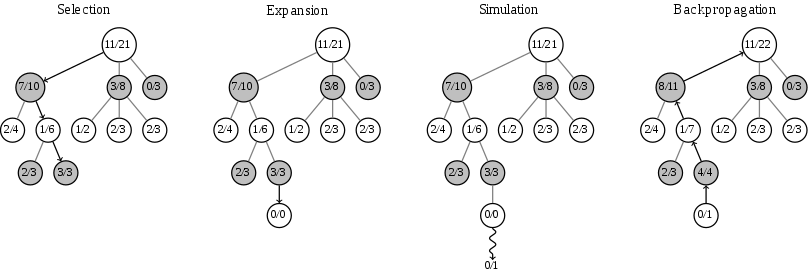
\includegraphics[width=0.6\linewidth]{./images/mcts.png}
      \caption{The four main components of MCTS}
    \end{figure}
  \end{itemize}
\end{frame}

%------------------------------------------------

%------------------------------------------------

\begin{frame}
  \frametitle{Bandit Algorithms on MCTS}

  \begin{itemize}
    \item In MCTS, sampling of the paths through the tree can be thought of as a multi-armed bandit problem
    \item MCTS is modeled like this because the finite/infinite horizon in MDPs is not enforced in certain decision trees
    \item This leads to the selection step following schemes like UCB, called UCT, which work well in practice
  \end{itemize}
\end{frame}

%------------------------------------------------

%------------------------------------------------

\begin{frame}
  \frametitle{Dynamic Programming Formulation of UCT}

  \begin{itemize}
      \item If we assume that the process is finite horizon, i.e. the process cannot loop through the same state ad infinitum, we can model MCTS as a lookahead policy from an MDP
      \item Recall the Bellman equation
        \begin{gather*}
          V_t(s) = \max_{a} R_a(S_{t+1}, S_t) + V(S_{t+1})
        \end{gather*}
      \item $S_t$ is the node in the tree, $a_t$ is an edge of the node, we can estimate $V_t(s)$ by sampling via UCT to get the lookahead policy
        \begin{gather*}
          \tilde{V}_t(\tilde{S_t}) = \max_{a} R_a(\tilde{S}_{t+1}, \tilde{S}_t) + \tilde{V}(\tilde{S}_{t+1}) + c_{uct} \sqrt{\frac{\ln N_(\tilde{S}_t)}{N(\tilde{S}_{t}, a)}}
        \end{gather*}
  \end{itemize}
\end{frame}

%------------------------------------------------

\section{AlphaZero}

%------------------------------------------------

\begin{frame}
  \frametitle{History of AlphaZero}

  \begin{itemize}
    \item 3 different versions each improving on itself
    \item AlphaGo (January 2016)
      \begin{itemize}
        \item Used supervised learning to learn an initial neural network then used self play for further training
      \end{itemize}
    \item AlphaGo Zero (October 2017)
      \begin{itemize}
        \item Removed the supervised learning part and engineering tricks of AlphaGo
        \item Went from two neural networks to just one
      \end{itemize}
    \item Alpha Zero (December 2017)
      \begin{itemize}
        \item Removes evaluation component of AlphaGo Zero and other engineering tweaks
      \end{itemize}
    \item In what follows, I will say Alpha Zero to mean both of the last two
  \end{itemize}
\end{frame}

%------------------------------------------------

%------------------------------------------------

\begin{frame}
  \frametitle{Overview of AlphaZero}

  \begin{itemize}
    \item I break AlphaZero into three main components
    \item Policy and Value Learning
      \begin{itemize}
        \item Comprises the neural network and the training part of the algorithm
      \end{itemize}
    \item Self Play
      \begin{itemize}
        \item The way that the algorithm generates data for the previous step
      \end{itemize}
    \item Evaluator
      \begin{itemize}
        \item Consists of the logic that determines which neural networks to keep and throw away
        \item Not in Alpha Zero
      \end{itemize}
  \end{itemize}
\end{frame}

%------------------------------------------------

%------------------------------------------------

\begin{frame}
  \frametitle{Policy and Value Learning}

  \begin{itemize}
    \item Structure of neural network:
      \begin{itemize}
        \item Residual block tower consisting of 40 blocks
        \item Output of tower is fed into two heads
        \item Value head produces a single value representing probability of winning
        \item Policy head outputs a vector of probability logits
      \end{itemize}
    \item Loss:
      \begin{gather*}
        (p, v) = f_\theta(S), \quad \ell = (z - v) - \pi^T \log p + c \lVert \theta \rVert^2
      \end{gather*}
    \item Uses batches of size 4,096 turns sampled from the previous 500,000 games
    \begin{figure}
      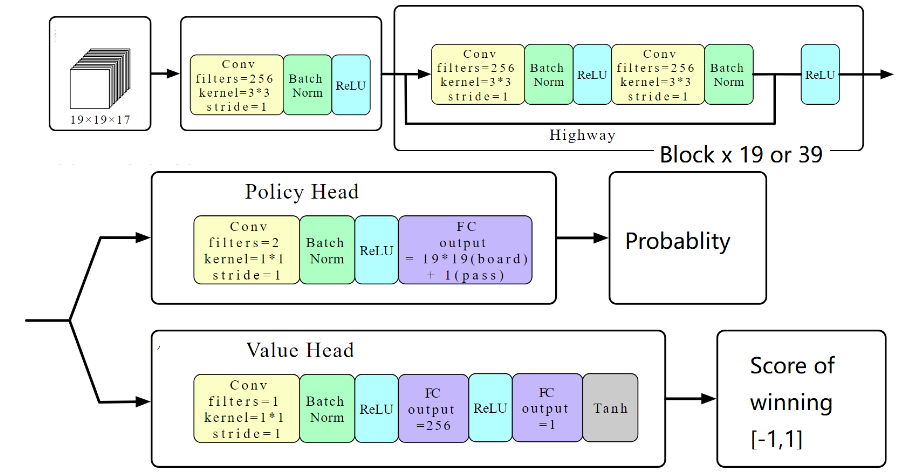
\includegraphics[width=0.38\linewidth]{./images/network.png}
      \caption{Diagram of network architecture}
    \end{figure}
  \end{itemize}
\end{frame}

%------------------------------------------------

%------------------------------------------------

\begin{frame}
  \frametitle{Reinforcement Through Self Play}

  \begin{itemize}
    \item Highly distributed set of games played through MCTS
    \item 800 rounds of MCTS performed using the following version of PUCT:
      \begin{gather*}
        a_{t'} = \max_a \frac{V(S_L)}{N(S_{t'})} + c_{puct} P(S_{t'}, a) \frac{\sqrt{\sum_a N(S_{t'}, a)}}{N(S_{t'})}
      \end{gather*}
    \item Final selection of action, if $t < 30$:
      \begin{gather*}
        \pi_a(S_t) = \frac{N(S_t, a)}{\sum_b N(S_t, b)}
      \end{gather*}
      Otherwise,
      \begin{gather*}
        \max_a \frac{N(S_t, a)}{\sum_b N(S_t, b)}
      \end{gather*}
    \item To encourage exploration, add Diriclet noise $\eta \sim $ Dirichlet(0.03) to $P(S_0, a)$
      \begin{gather*}
        P(S_t, a) = (1-\epsilon)P(S_t, a) + \epsilon \eta
      \end{gather*}
  \end{itemize}
\end{frame}

%------------------------------------------------

%------------------------------------------------

\begin{frame}
  \frametitle{Evaluating}

  \begin{itemize}
    \item After a 1,000 training iterations, it is time to evaluate the network to see if it is better
    \item Using the checkpoint, play 400 games with reduced exploration
      \begin{itemize}
        \item if the checkpoint beats the previous best 55\% of the time, it becomes the new best and update the self play networks
        \item Otherwise do nothing
      \end{itemize}
    \item This part is removed in AlphaZero but is still useful to calculate ELO at this stage
  \end{itemize}
\end{frame}

%------------------------------------------------

%------------------------------------------------

\begin{frame}
  \frametitle{Putting it All Together}

  \begin{figure}
    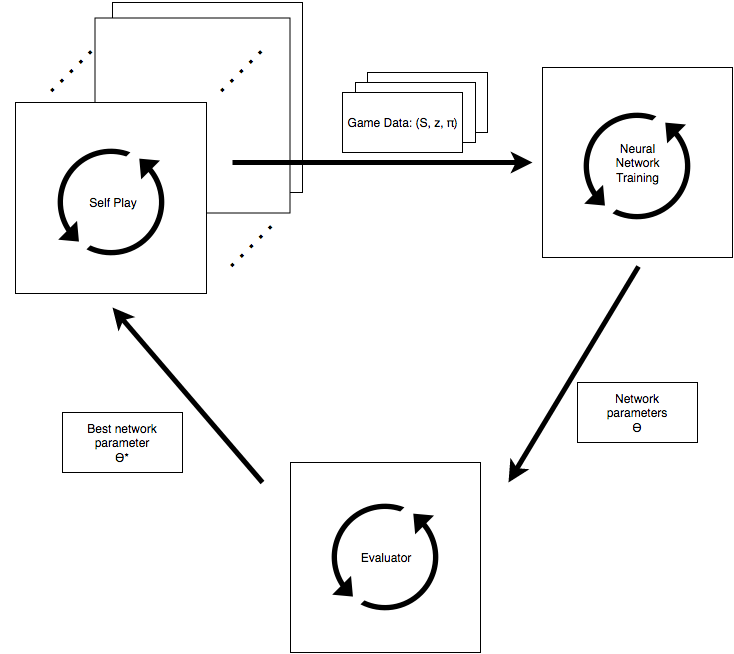
\includegraphics[width=0.61\linewidth]{./images/alphazero.png}
    \caption{High level block diagram of AlphaZero}
  \end{figure}
\end{frame}

%------------------------------------------------

%------------------------------------------------

\begin{frame}
  \frametitle{Mathematical Formulation of AlphaZero}

  We can model AlphaZero as an MDP with the following parameters:
  \begin{itemize}
    \item $S_t = (X_t, B_t)$, the state consists of the physical game state $X_t$ and the belief state of the correct policy ($\bar{P}_{X_t}(\cdot)$) and value ($\bar{V}_{X_t}$) at node $X_t$ which is given by our neural network $(\bar{P}_{X_t}(\cdot),\bar{V}_{X_t}) = f_\theta(X_t)$
    \item Action space is all possible moves, possibly encoded
    \item No transition probabilities, everything is deterministic
    \item Reward $R_a(S_{t+1}, S_t)$ is 0 if nothing or a draw occurs, 1 if you win, and -1 if you lose
    \item You can then view the MCTS in AlphaZero as a stochastic lookahead policy for the stochastic dynamic program of playing the game
  \end{itemize}
\end{frame}

%------------------------------------------------

\section{Current Work}

\subsection{Motivation}

%------------------------------------------------

\begin{frame}
  \frametitle{Motivation: AlphaZero and Action Space}

  \begin{itemize}
    \item AlphaZero handles large state spaces really well due to the neural network
    \item However, network outputs a policy vector which can get quite large
    \item UCT exploration policy is determined by value so they seem intrinsically tied
  \end{itemize}
\end{frame}

%------------------------------------------------

%------------------------------------------------

\begin{frame}
  \frametitle{Motivation: Chess Example}

  \begin{columns}[T]
    \begin{column}{.48\textwidth}
      \textbf{Input States}
      Tensor of 8x8x119
      \begin{itemize}
        \item 6 - positions for white pieces, 6 - positions for black pieces, 2 - keeps track of repetitions
        \item Repeated 8 times for a 8-step history
        \item 7 of more planes to keep track of player, castling, etc.
      \end{itemize}
    \end{column}
    \hfill
    \begin{column}{.48\textwidth}
      \textbf{Output Policy}
      Tensor of 8x8x73 which represents picking a square and moving it to one of 73 possible different moves
      \begin{figure}
        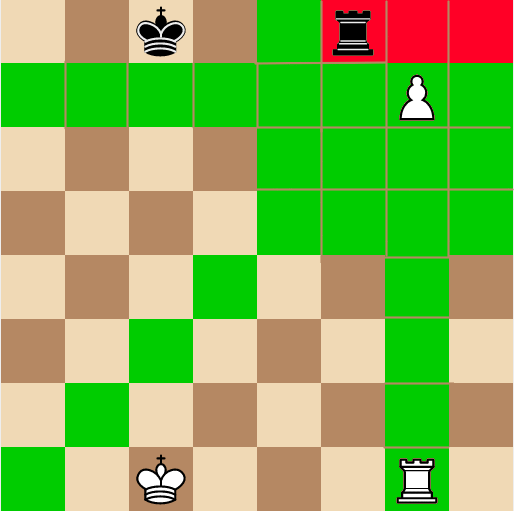
\includegraphics[width=0.5\linewidth]{./images/possible-moves.png}
        \caption{How AlphaZero encodes chess moves}
      \end{figure}
    \end{column}
  \end{columns}
\end{frame}

%------------------------------------------------

%------------------------------------------------

\begin{frame}
  \frametitle{Motivation: Scrabble}

  \begin{itemize}
    \item Scrabble represents an interesting case. On one hand, MCTS with classical AI heuristics became super human in the early 2000's. Now, a more sophisticated algorithm based on MCTS could not even load into memory
    \item Why? Must encode for every possible Scrabble move possible, with 100,000 English words and 15x15 board, intractable
  \end{itemize}

  \begin{figure}
    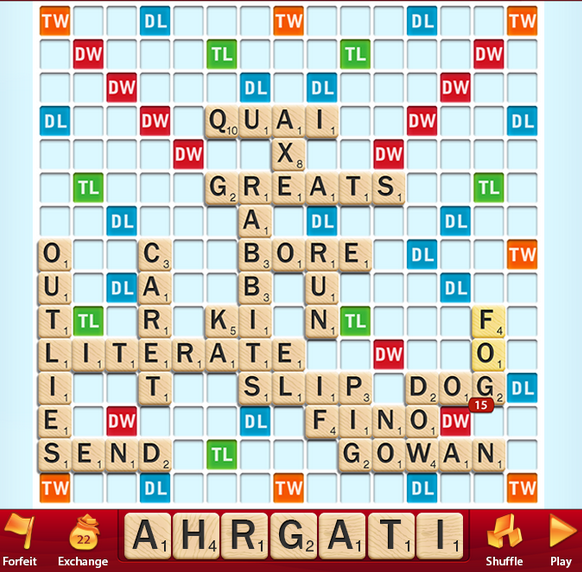
\includegraphics[width=0.29\linewidth]{./images/scrabble.png}
    \caption{Scrabble Board}
  \end{figure}
\end{frame}

%------------------------------------------------

%------------------------------------------------

\begin{frame}
  \frametitle{Motivation: Potential Solution}

  \begin{itemize}
    \item Must get rid of the policy component of the neural network
      \begin{gather*}
        (v, \xcancel{p}) = f_\theta{(s)}
      \end{gather*}
    \item Couple of different ways:
      \begin{itemize}
        \item Use a MCTS lookahead policy that does not rely on a prior distribution (what I've done)
        \item Induce a prior probability distribution based on the values of the next states
      \end{itemize}
    \item Added benefit of much more simple computations in the neural network
  \end{itemize}
\end{frame}

%------------------------------------------------

\subsection{Progress}

%------------------------------------------------

\begin{frame}
  \frametitle{Framework Overview}

  \begin{itemize}
    \item The framework that I am developing to experiment is modular in several different aspects:
      \begin{itemize}
        \item Games can be easily added via a standard interface
        \item Different MCTS variations can be added via a standard interface
      \end{itemize}
    \item Allows for quicker prototyping and experimentation
    \item The core of the framework interfaces with the above, does not use game/mcts specific implementation
  \end{itemize}
\end{frame}

%------------------------------------------------

%------------------------------------------------

\begin{frame}
  \frametitle{Framework Progress}

  \begin{itemize}
    \item Current implementation: $>$2,000 LOC
    \item Over 5,000 LOC written during development
    \item Everything runs on a local machine: self play using MCTS framework and training through tensorflow
    \item Distributive interface implemented through a ZMQ server with database storage
  \end{itemize}
\end{frame}

%------------------------------------------------

%------------------------------------------------

\begin{frame}[fragile]
  \frametitle{Game Class}

  \begin{lstlisting}[basicstyle=\tiny, showstringspaces=false, language=Python]
  class Game:

  def generate_moves(self):
    raise NotImplementedError("Generate moves not implemented")

  def transition(self):
    raise NotImplementedError("Transition not implemented")

  def set_state(self):
    raise NotImplementedError("Set state not implemented")

  def visualize(self):
    raise NotImplementedError("Visualize not implemented")
  \end{lstlisting}
\end{frame}

%------------------------------------------------

%------------------------------------------------

\begin{frame}[fragile]
  \frametitle{MCTS Class}

  \begin{lstlisting}[basicstyle=\tiny, showstringspaces=false, language=Python]
  class MCTS:

  def __init__(self, root, game, node_config):
      self.tree = Tree(root, node_config)
      self.game = game
      self.node_config = node_config

  def selection(self):
    raise NotImplementedError("Selection not implemented")

  def expansion(self):
    raise NotImplementedError("Expansion not implemented")

  def simulation(self):
    raise NotImplementedError("Simlation not implemented")

  def backpropagation(self):
    raise NotImplementedError("Backpropagation not implemented")

  def selection_final(self):
    raise NotImplementedError("Final selection not implemented")

  def run(self):
    raise NotImplementedError("Run not implemented")
  \end{lstlisting}
\end{frame}

%------------------------------------------------

%------------------------------------------------

\begin{frame}
  \frametitle{Parallel Architecture}
  For distributive performance, the framework breaks the tasks into workers for the major components of AlphaZero
  \begin{itemize}
    \item Self Play Worker
    \item Training Worker
    \item Oracle Worker
    \item Evaluator Worker
  \end{itemize}
  \begin{figure}
    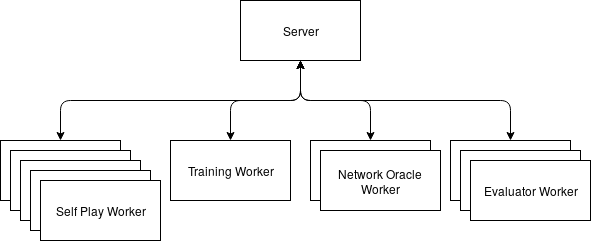
\includegraphics[width=0.5\linewidth]{./images/architecture.png}
    \caption{Block Diagram of Architecture}
  \end{figure}
\end{frame}

%------------------------------------------------

%------------------------------------------------

\begin{frame}
  \frametitle{Technical Difficulties: Distributive Computing}

  \begin{itemize}
    \item Distributive computing is hard in general when the processes must communicate
    \item The ZMQ architecture works very well but is the communication overhead worth it?
    \item Might be requried due to the Global Interpreter Lock in CPython
  \end{itemize}
\end{frame}

%------------------------------------------------

%------------------------------------------------

\begin{frame}
  \frametitle{Technical Difficulties: Differences with AlphaZero}

  \begin{itemize}
    \item Google has access to far greater computational resources than Princeton and so their algorithm has a slightly different architecture
    \item Google has access to TPUs further enhancing their performance
    \item Each self play worker has their own copy of the network
      \begin{itemize}
        \item No need for oracle worker
        \item Much faster for MCTS iterations
      \end{itemize}
    \item Google most likely implemented it in C++ for better speed
  \end{itemize}
\end{frame}

%------------------------------------------------

%------------------------------------------------

\begin{frame}
  \frametitle{Technical Difficulties: Hyperparameters}

  \begin{itemize}
    \item Many different hyperparameters to tune and might be game/network specific
    \item MCTS hyperparameters:
      \begin{itemize}
        \item $C_{uct}$ - for UCT algorithm which is the exploration-exploitation tradeoff
        \item $\gamma$ - for EXP3 defines mixture of sampling distributions
      \end{itemize}
    \item Exploration hyperparameters
      \begin{itemize}
        \item $\tau$ - number of turns that the final MCTS selection will sample randomly 
        \item $\epsilon$ - Amount of Dirichlet noise to add to root to encourage exploration/non-deterministic play
      \end{itemize}
    \item Loss weights
  \end{itemize}
\end{frame}

%------------------------------------------------

%------------------------------------------------

\begin{frame}
  \frametitle{Proof of Concept: Pawns}

  \begin{itemize}
    \item Simplified version of chess where there are only pawns and the goal is to be the first one to get a pawn to the end
    \item Ran both AlphaZero and my version with EXP3 for 1,000,000 training iterations
    \item Both develop more complicated structures as time progresses
  \end{itemize}
\end{frame}

%------------------------------------------------

\section{Demo}

%------------------------------------------------

\begin{frame}
\frametitle{Demo}
  \begin{center}
    \Large Demo Time
    \end{center}
\end{frame}

%------------------------------------------------

\section{Next Steps and Future Directions}

%------------------------------------------------

\begin{frame}
  \frametitle{Next Steps: Low Hanging Fruit}

  \begin{itemize}
    \item Make code more performant in the MCTS loop
      \begin{itemize}
        \item AlphaZero 0.4s vs. 4s
        \item AlphaZero 800 rollouts vs. 100
      \end{itemize}
    \item Optimize the parallelization
    \item Add more complicated games and validate
    \item Refactor code to make more modular
  \end{itemize}
\end{frame}

%------------------------------------------------

%------------------------------------------------

\begin{frame}
  \frametitle{Next Steps: Compute Cluster}

  \begin{itemize}
    \item Write slurm wrapper for the framework
    \item Need to refactor optimization code to allow splitting of batches across multiple GPUs
    \item Predict that I will be able to get the framework doing 500 games per second on 1,000 CPUs which matches the production of AlpheZero
  \end{itemize}
\end{frame}

%------------------------------------------------

%------------------------------------------------

\begin{frame}
  \frametitle{Next Steps: ELO Evaluation}

  \begin{itemize}
    \item Standard in all of the AlphaZero papers
    \item Two ways ELO calculation can be done:
      \begin{enumerate}
        \item Using the formula:
          \begin{gather*}
            \mathbb{P}(a \text{ beats } b) = \frac{1}{1 + e^{c_{elo} (R_b - R_a)}}
          \end{gather*}
        \item Using techniques that take into account cross-play
      \end{enumerate}
  \end{itemize}
\end{frame}

%------------------------------------------------

%------------------------------------------------

\begin{frame}
  \frametitle{Next Steps: Scrabble}

  \begin{itemize}
    \item The ultimate goal of the project
    \item Generating moves presents a much harder challenge than the other games
    \item Pre existing libraries written in C++ through Quackle
  \end{itemize}
  \begin{figure}
    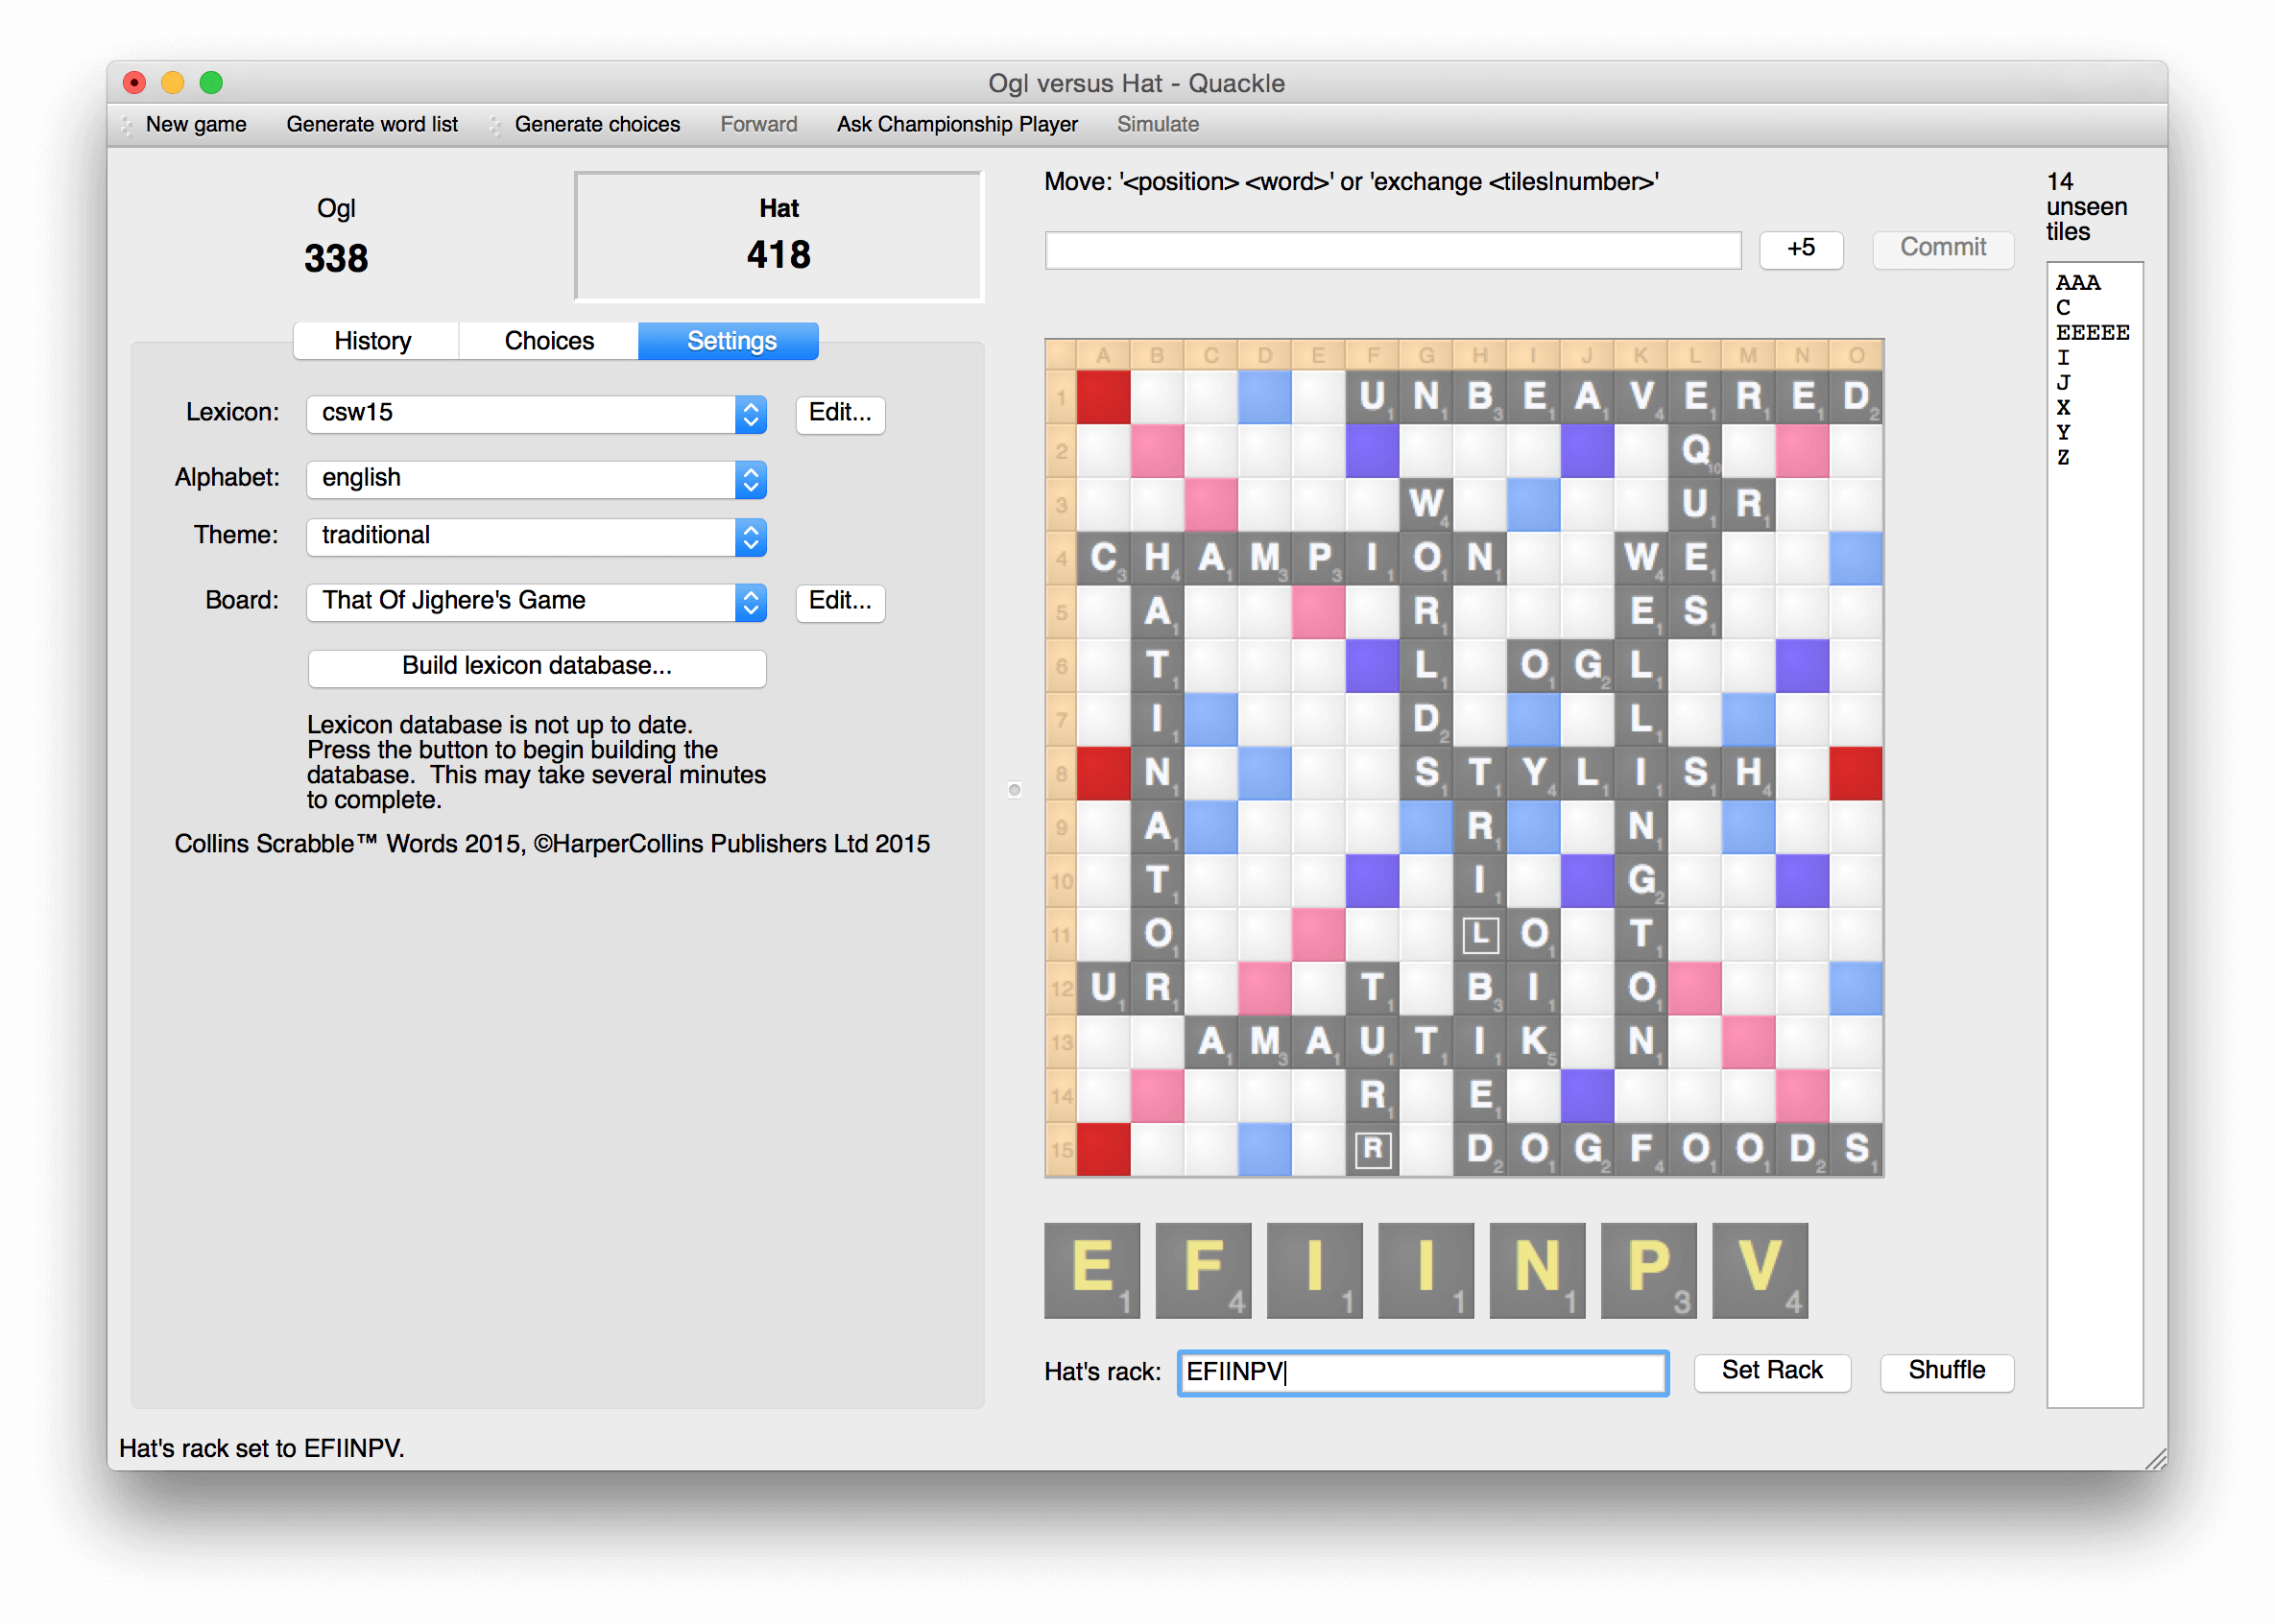
\includegraphics[width=0.5\linewidth]{./images/quackle.png}
    \caption{Quackle Environment}
  \end{figure}
\end{frame}

%------------------------------------------------

%------------------------------------------------

\begin{frame}
  \frametitle{Future Directions: Robotics}

  \begin{columns}[T]
    \begin{column}{.48\textwidth}
      \begin{itemize}
        \item The algorithm is well suited for the world of robotics - large state space and many actions
        \item MuJoCo is an open source environment from the University of Washington that is widely used to benchmark control algorithms
      \end{itemize}
    \end{column}
    \hfill
    \begin{column}{.48\textwidth}
      \begin{figure}
        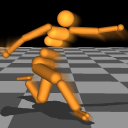
\includegraphics[width=0.5\linewidth]{./images/mujoco.png}
        \caption{MuJoCo physics environment}
      \end{figure}
    \end{column}
  \end{columns}
\end{frame}

%------------------------------------------------

%------------------------------------------------

\begin{frame}
  \frametitle{Future Directions: Multiplayer Games}

  \begin{itemize}
    \item Prior work on UCT applied to multiplayer games show that the the strategy extracted from UCT is a mixed strategy equilibrium
    \item Avenue of research, enhancing AlphaZero with online learning to exploit a suboptimal player
    \item Halite II would be a good game to tackle
  \end{itemize}

  \begin{figure}
    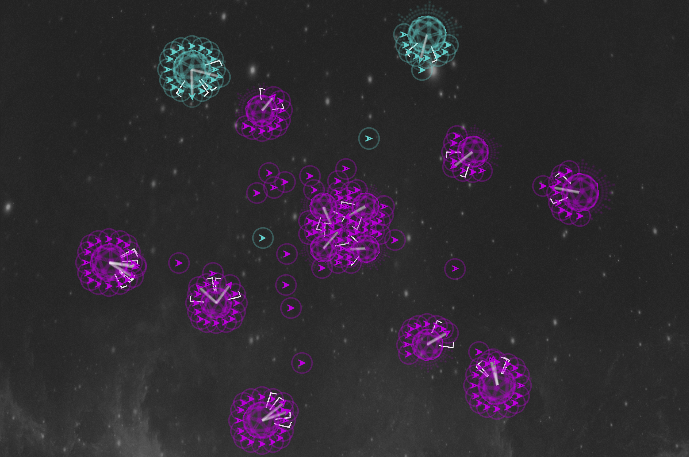
\includegraphics[width=0.45\linewidth]{./images/halite.png}
    \caption{A game of Halite II in progress}
  \end{figure}
\end{frame}

%------------------------------------------------

%------------------------------------------------

\begin{frame}
  \frametitle{Future Directions: SmartDriving Cars}

  \begin{itemize}
    \item Following the work done by Chenyi, this could be extended to learning how to drive from the use of the TORCS environment
    \item Chenyi had to manually drive car simulator to generate his data
    \item Chenyi showed that the results work surprisingly well when transfering from simulator to real world
  \end{itemize}
  \begin{figure}
    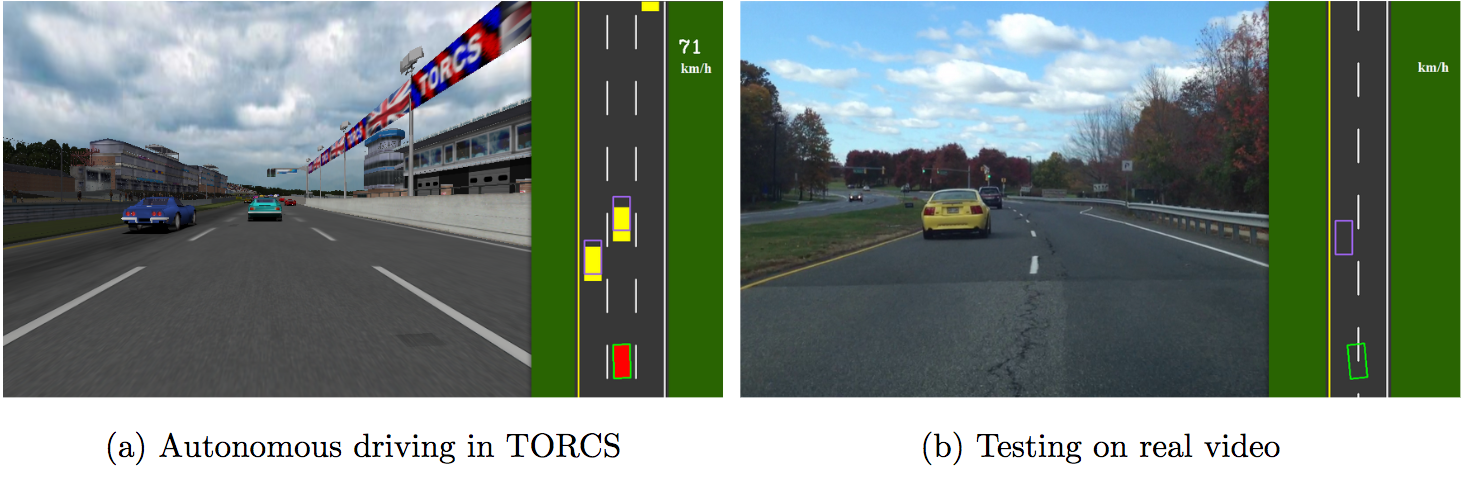
\includegraphics[width=0.8\linewidth]{./images/torcs.png}
    \caption{Chenyi's work in a simulator and real environment}
  \end{figure}
\end{frame}

%------------------------------------------------

%------------------------------------------------

\begin{frame}
  \frametitle{Future Directions: Real World Applications}

  \begin{itemize}
    \item Method is capable of being applied to anything with a simulator that can generate ``self-play'' data
    \item Interested in working with Warren in any domain that he sees the benefit of using a AlphaZero like algorithm
    \item Examples: optimizing electrical network flow, telecom networks, automatic circuit design
  \end{itemize}
\end{frame}

%------------------------------------------------

%------------------------------------------------

\begin{frame}
  \frametitle{Goals for PhD}

  \begin{itemize}
    \item A mixture of applications and theory in the realm of reinforcement learning/deep reinforcement learning
    \item Working on how to reduce the dependence on the size of the action space
    \item Hierarchichal learning - how to group actions together to form a hierarchy of decisions/goals
  \end{itemize}
\end{frame}

%------------------------------------------------

%----------------------------------------------------------------------------------------

\end{document}